Our design consists of three major parts: modifying the existing DNN models to provide more information, modifying the open source labeling tool \textit{labelme} to provide a customized Graphical User Interface, and deploying our tool online with restriction policy.

\subsection{Modifying DNN Models}
In this part, we will integrate three different DNN models to solve three problems: object detection, semantic segmentation and human gesture detection in order to facilitate the annotation process. In specific, we decide to use YoloV3, DeepLabV3 and PAF model to conquer those problems correspondingly. Given the dataset from HJ Drive, we will first train the models in python environment and then transfer the trained models to our C++ Keras framework to integrate to our QT-based semi-annotation tool.

\subsection{Customizing GUI}
In this part, we will modify the GUI interface of \textit{labelme} to make it more convenient for users and to incorporate the extra information obtained from the first part. Specifically, we will add sub-tag mechanism to reasonably and clearly categorize all the tags and provide different colors for different kinds of tags. And we will create an interface for displaying middle step results and clearly distinguish them with normal annotation.

\subsection{Online Deployment}
In this part, we will deploy our tool online. The major goal of online deployment is to protect the raw data sets from being distributed without intention. With the online deployment, when outsourcing, we don't need to hand over the entire data set, but we can store the data in our backend database and restrict user access to these data. Our work here is to port our GUI in the second part to the web frontend and establish a backend database and computing logic to perform the automated annotation in the first part.

\subsection{Specific Engineering Requirements}
According to the requirement from our customer, our annotation tool should put emphasis on accuracy and efficiency of labeling. Besides, we are given freedom to modify the Labelme source codes to make it more user-friendly. Therefore base on those requirement, we have interpreted them to a series engineering specifications:
\begin{enumerate}
    \item Label Efficiency. The average time that takes a common worker to label one image using annotation tool. This value should be limited to 60 seconds.
    \item DNN Preprocessing Accuracy. The accuracy of annotation tag suggested by our DNN model. It should be higher than 90\%.
    \item Percentage of Labeled Pictures. The relative percentage of pictures that are labeled compared to the number of all input image. This value reflects the coverage of DNN models. The average value should be at least higher than 65\% for a set of images taken from the on-board system. 
    \item Depth of Label Hierarchy. The depth of tag hierarchy generated by our annotation tool. The average value of this value should larger than 2 to indicate our success in simplifying the tag categories.
    \item Budget of Project. Our budget is within 1000 RMB.
\end{enumerate}

\begin{table}[H]
\begin{tabular}{|l|l|}
\hline
\textbf{Engineering Specification} & \textbf{Quantity[Units]} \\ \hline
Label Efficiency & $\leq60$[s] \\ \hline
DNN Preprocessing Accuracy & $\geq90$\% \\ \hline
Percentage of Labeled Pictures & $\geq65\%$ \\ \hline
Depth of Label Hierarchy & $\geq2$ \\ \hline
Budget of Project & $\leq1000$[\yen] \\ \hline
\end{tabular}
\caption{Engineering Specification}
\label{tab:quantification}
\end{table}
\subsection{Quality Function Deployment}
Including all the customer requirements and engineering requirements, we collect the information and create the QFD chart in Fig. \ref{fig:qfd}. We consider high labeling speed and high labeling coverage as the two most important customer requirements. Road object detection and pedestrian gesture predication also play significant roles. The weight is graded and 10 represents the highest demand while 1 represents a lowest one. We transfer this information into the engineering requirements with quantified terms, and list them on the top of the chart. In the middle part, we score the correlation between customer requirements and engineering specifications. 9 represents a strong relationship, 3 represents a medium one and 1 means a small relationship. If there is a blank, it means no relation exists between these two.

Then, we multiply the scores between corresponding quantified and unquantified requirements to obtain the total scores. The measurements units, normalized scores and rank orders are also shown with the total scores at the bottom of the chart. We place the competitive benchmark - Labelme at the right of the chart and score it with the listed customer requirements. In addition to these, the engineering specifications have potential correlation between themselves. Therefore, we put the evaluation in the top triangle. The '+' symbol shows a positive relation while '-' shows negative one. 
\begin{figure}[htbp]
  \centering 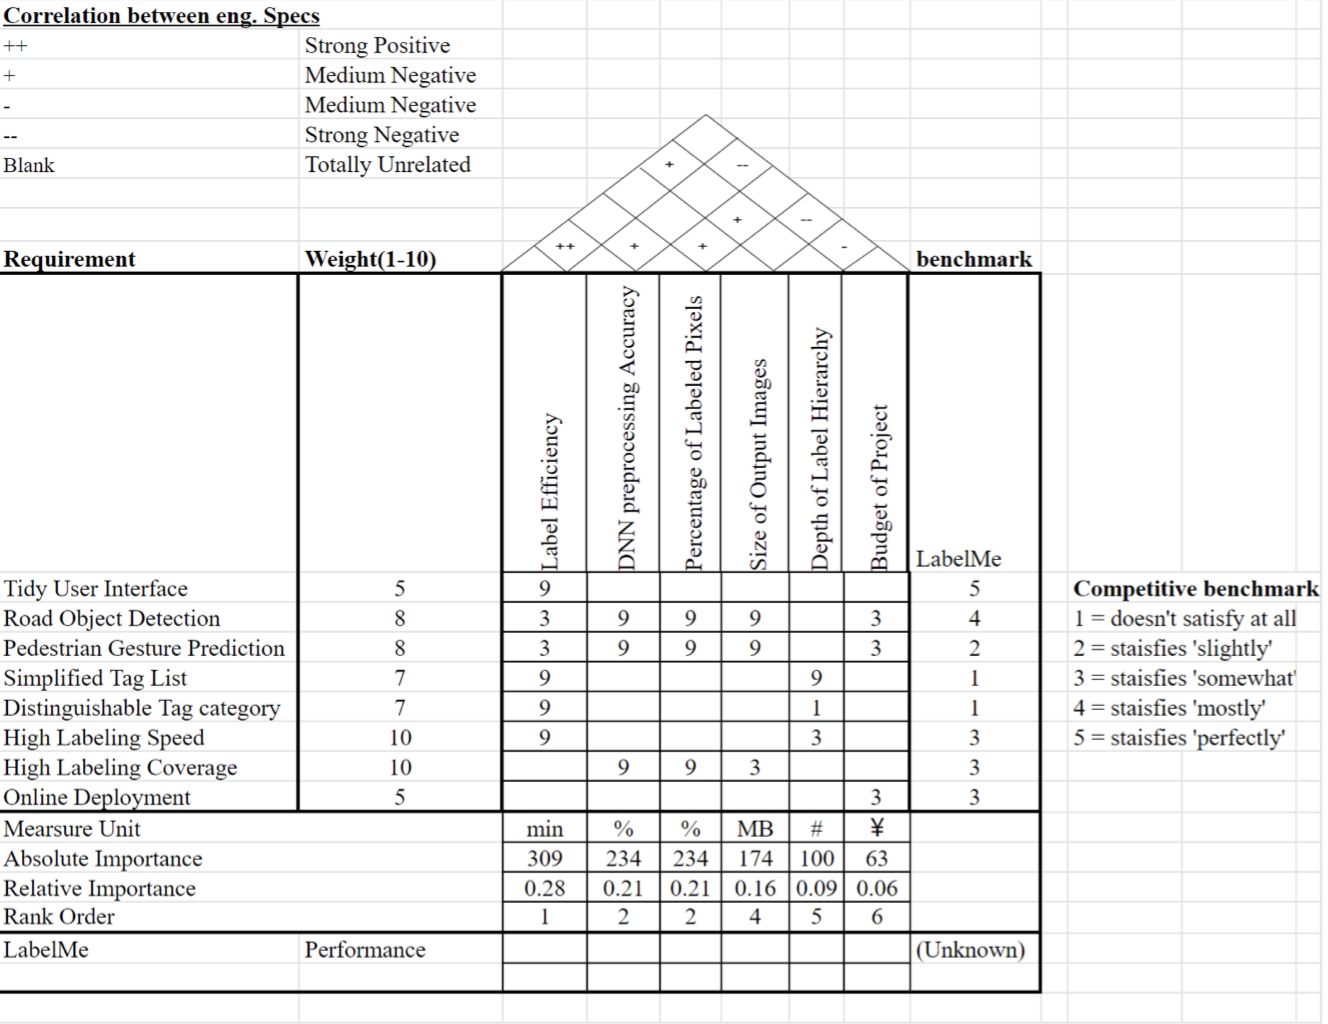
\includegraphics[width=\linewidth]{qfd2.png} % insert QFD here
  \caption{Quality Function Deployment}
  \label{fig:qfd}
\end{figure}


